\section{Evaluation}

We use ChampSim~\cite{champsim}, an open-source trace-driven simulator, to evaluate the efficacy of BTB-X on server workload traces provided for the first Instruction Prefetching Championship (IPC-1)~\cite{ipc1}. The modeled processor resembles Intel Sunny Cove~\cite{sunnycove}. We compare the storage requirements and performance of BTB-X against a conventional BTB design (Conv-BTB) that stores full target addresses, and also against the state-of-the-art BTB design, called PDede~\cite{pdede}, which stores compressed targets.

\subsection{Storage comparison}
\Cref{pact:table:storageComp} presents the number of branches the different BTB organizations (BTB-X, PDede, and Conv-BTB) can track at different storage budgets. The storage budgets shown are BTB-X storage required for storing 256, 512, 1K, 2K, 4K, 8K, and 16K branches. Our calculations assume a 48-bit virtual address space. As the table shows BTB-X stores significantly more branches than any other BTB organizations. Concretely, it stores 2.24x more branches than a conventional BTB organization. Compared to PDede, BTB-X stores 1.24x more branches at 0.9KB storage budget and 1.34x more branches at 58KB storage budget. BTB-X's advantage over PDede increases with storage budget because PDede entry size increases with the number of branches PDede can accommodate. 

\subsection{Performance comparison}
\Cref{pact:fig:perf} presents the performance gains obtained by different BTB designs on a set of server workloads. The results are normalized to the performance of Conv-BTB with 0.9KB storage budget. Instruction prefetching (FDIP) is enabled in all designs including the baseline. As the figure shows BTB-X provides significantly higher performance than the Conv-BTB and PDede for equal storage budgets of up to 29KB and 14.5KB respectively. For instance, BTB-X provides 45\% performance gain over the baseline compared to 38\% and 27\% of PDede and Conv-BTB, respectively, at 14.5KB budget. At large BTB storage budgets, the branch working sets of many workloads start to fit in the available BTB capacity, at which point the performance gap between BTB-X and the other two designs diminishes. A key take-away from this figure is that BTB-X outperforms the conventional BTB even when it is given just half the storage budget of its conventional counterpart. For example, in \Cref{pact:fig:perf}, the Conv-BTB improves performance by 27\% with a 14.5KB budget whereas BTB-X provides a 31\% improvement with just 7.25KB of storage. The reason for this behaviour is that BTB-X accommodates 2.24x more entries than Conv-BTB of equal storage budget; thus, halving BTB-X's budget still gives a slight capacity advantage over Conv-BTB.

\begin{small}
\begin{table}[t!]
  \centering
  \caption{Number of branches in different BTB designs.}
  \vspace{-0.1in}
  \label{pact:table:storageComp}
  \begin{tabular}{llrr} \hline
    \textbf{Storage} & \textbf{BTB-X (+ BTB-XC)} & \textbf{PDede}
    & \textbf{Conv-BTB} \\\hline
    0.9KB & 256 (+ 4) & 210 & 116\\\hline
    1.8KB & 512 (+ 8) & 415 & 232\\\hline
    3.6KB & 1K (+ 16) & 820 & 464\\\hline
    7.25KB & 2K (+ 32) & 1617 & 928\\\hline
    14.5KB & 4K (+ 64) & 3190 & 1856\\\hline
    29KB & 8K (+ 128) & 6292 & 3712\\\hline
    58KB & 16K (+ 256) & 12405 & 7424\\\hline
  \end{tabular}
  \vspace{-0.1in}
\end{table}
\end{small}

\begin{figure}[t!]
    \centering
    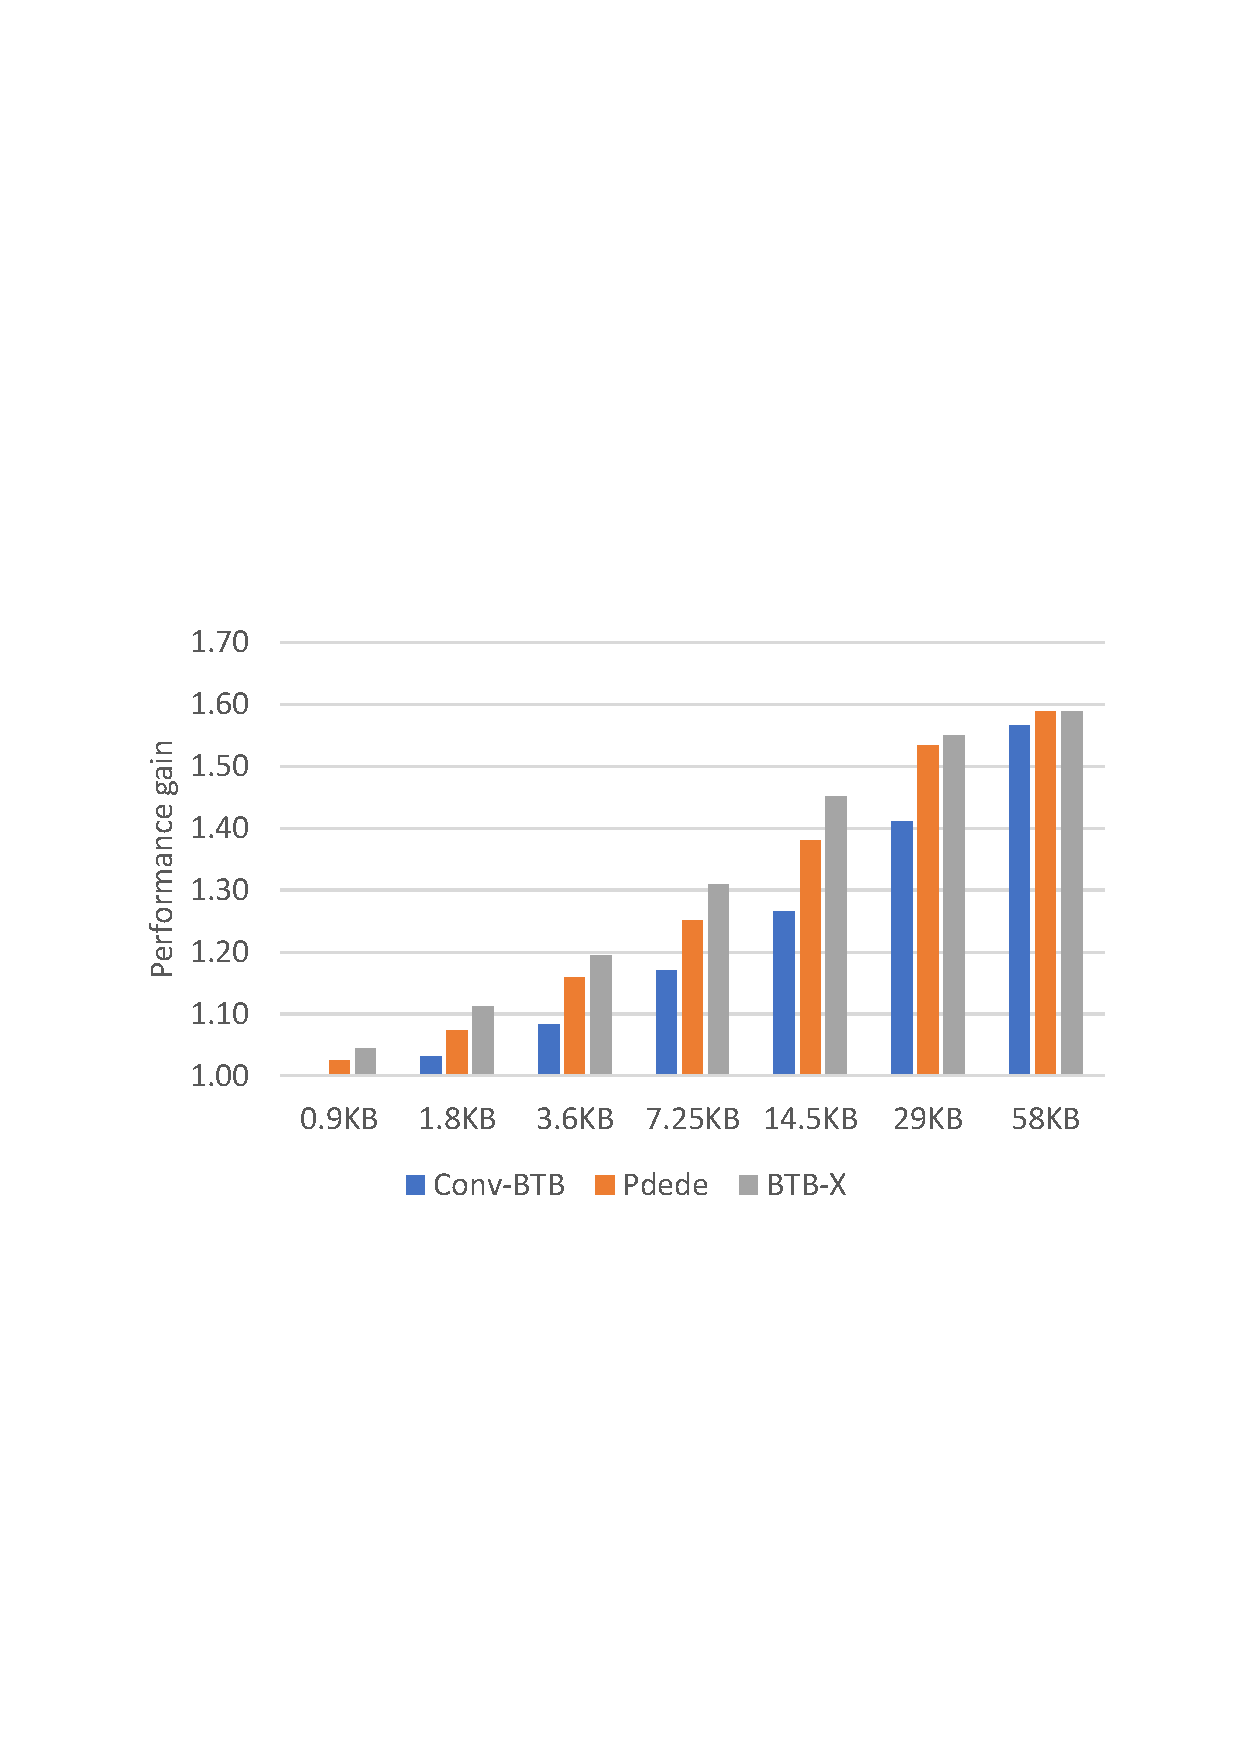
\includegraphics[width=0.9\columnwidth, trim=70 265 70 330, clip]{figures/ISOStorage-Server.pdf}
    \vspace{-0.1in}
    \caption{Performance comparison of different BTB designs.}
    \vspace{-0.1in}
    \label{pact:fig:perf}
\end{figure}